\clearpage
\section{Closure tests and systematic uncertainties on transfer factors\label{sec:bkgd-syst}}

Limitations in simulating detector effects and event kinematics 
requires us to apply appropriate systematics uncertainties 
on the simulation-based translation factors.  The following section 
describes how we obatain these systematic uncertainty through the 
method of closure tests.
%Since the transfer factors are obtained from simulation, an
%appropriate systematic uncertainty is assigned to each factor to
%account for theoretical uncertainties~\cite{Bern:2011pa} and
%limitations in the simulation modelling of event kinematics and
%instrumental effects. This section describes how the systematic
%uncertainties are determined from closure tests in data.

\subsection{Closure tests\label{sec:closure-tests-desc}}

At its core, the method compares an observed yield (\nobs) and a predicted
yield (\npre) in a sub-sample of a control region.  The predicted yield is constructed
by translating from a statisically independent data sample to the data sample of
interest by the use of the proper translation factor.  For example, for a given HT bin,
a prediction for the \njethigh, \nb=1, \mj sample can made by translating from the
\njetlow, \nb=1, \mj in data via the translation factor: 
\begin{equation}
  \label{equ:tf-ratio-closure}
  \frac{N_{\rm MC}^{\rm \mj}(\scalht,\njethigh, \nb=1)}{N_{\rm MC}^{\rm \mj}(\scalht,\njetlow,\nb=1)} 
\end{equation}

The agreement betwen \nobs and \npre is expressed as $(\nobs - \npre)/\npre$.
Assuming only statistical uncertainties on \nobs and \npre, deviation of the 
ratio from zero defines our level of closure. A closure test set is defined
as ratios for each \scaleht. Looking at the ratio as a function
of \scaleht allows the measurment of statistical significant biases from zero and/or 
any dependence on \scaleht.  If statistically significant biases
are observed, further studies are required to understand and correct
for these biases.

Eight sets of closure tests probe key ingredients of the simulation modelling 
of the SM backgrounds with genuine \met as a function of \scalht, as shown in
Fig.~\ref{fig:closure}. This is done for the two jet multiplicity bins
separately: (a) $2 \leq \njet \leq 3$ and (b) $\njet \geq 4$.

Under the assumption of closure for the full ensemble of tests,
systematic uncertainties on the transfer factors are derived for each
\njet category and \scalht regions. The treatment for
estimating the systematic uncertainties on the transfer factors is
described in Section~\ref{sec:syst-from-closure}.

\begin{figure}[h!]
  \begin{center}
    \subfigure[$2 \leq \njet \leq 3$]{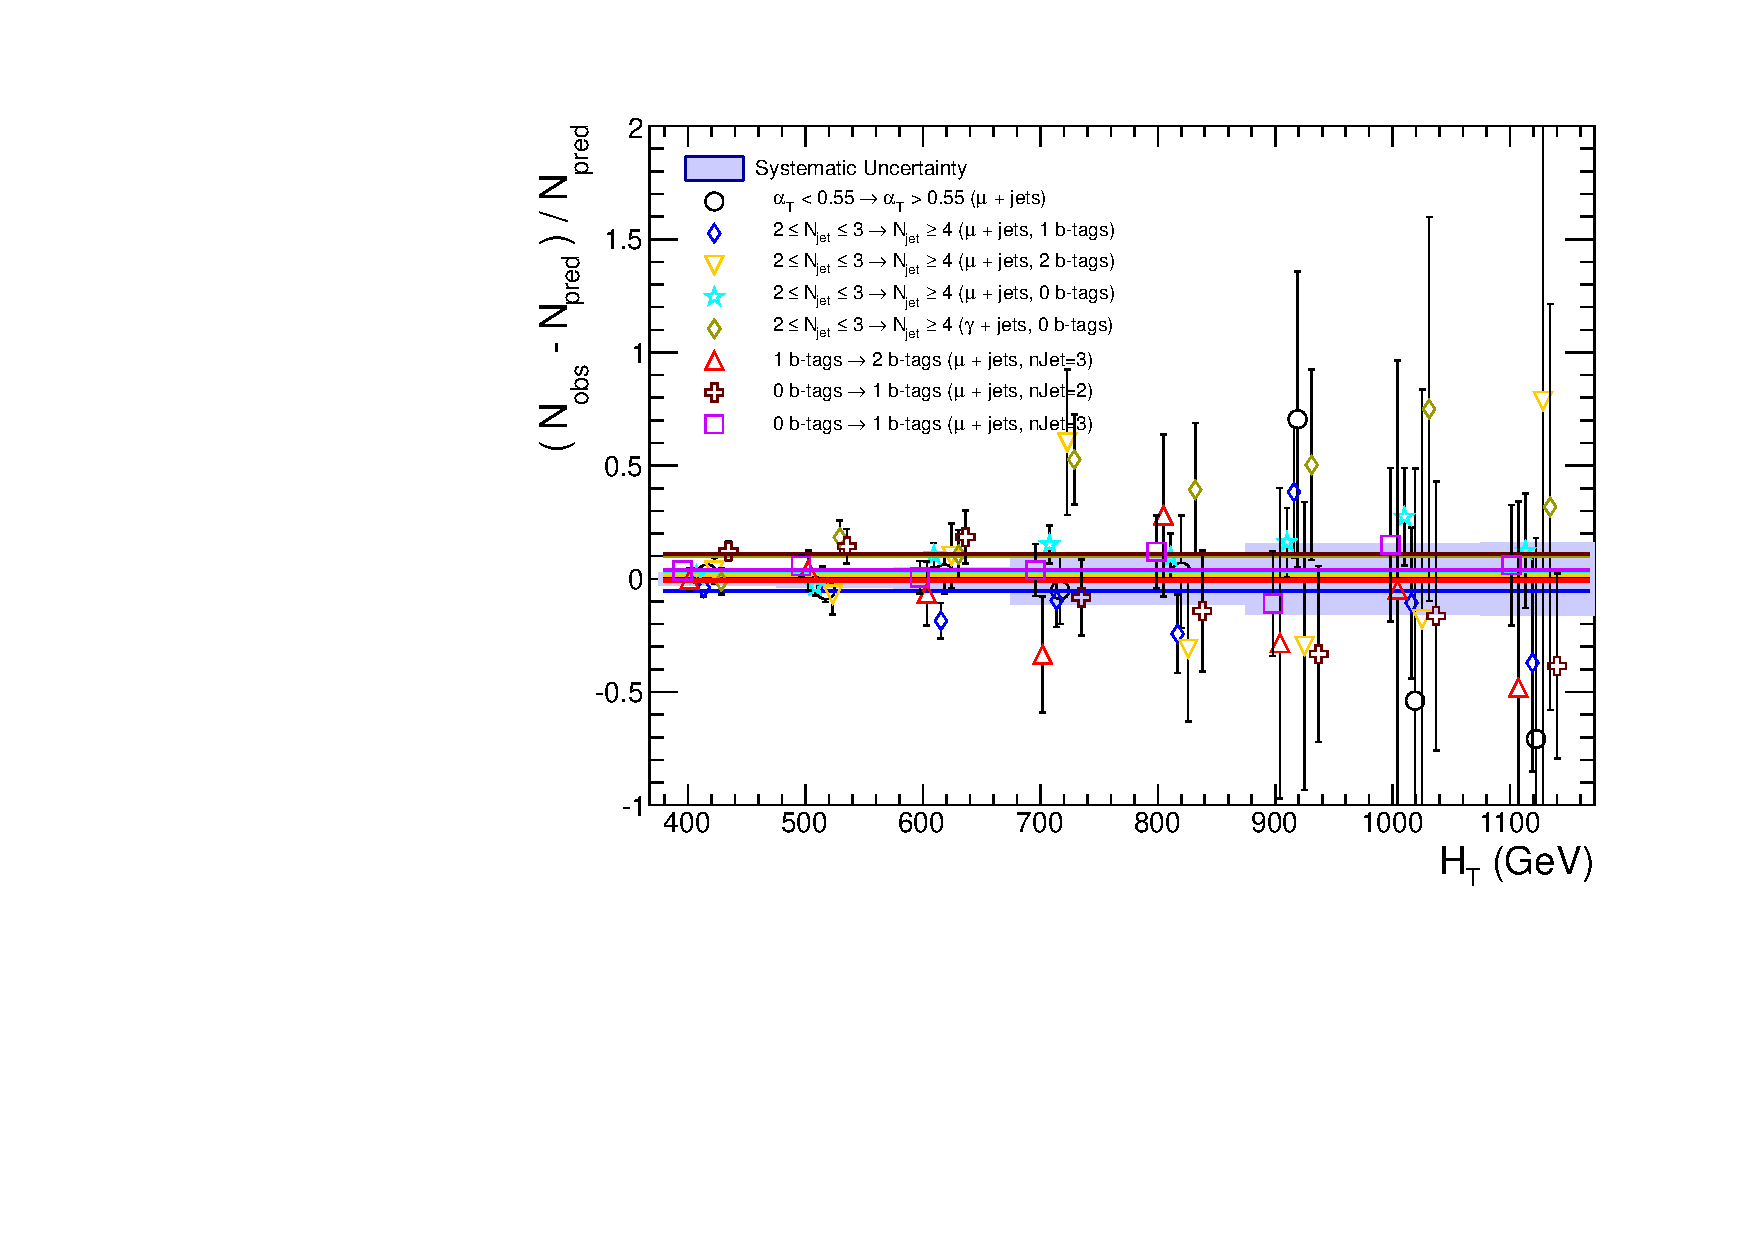
\includegraphics[width=0.7\textwidth]{figures/syst/closureTests_pf_take21_le3j.pdf}} \\
    \subfigure[$\njet \geq 4$]{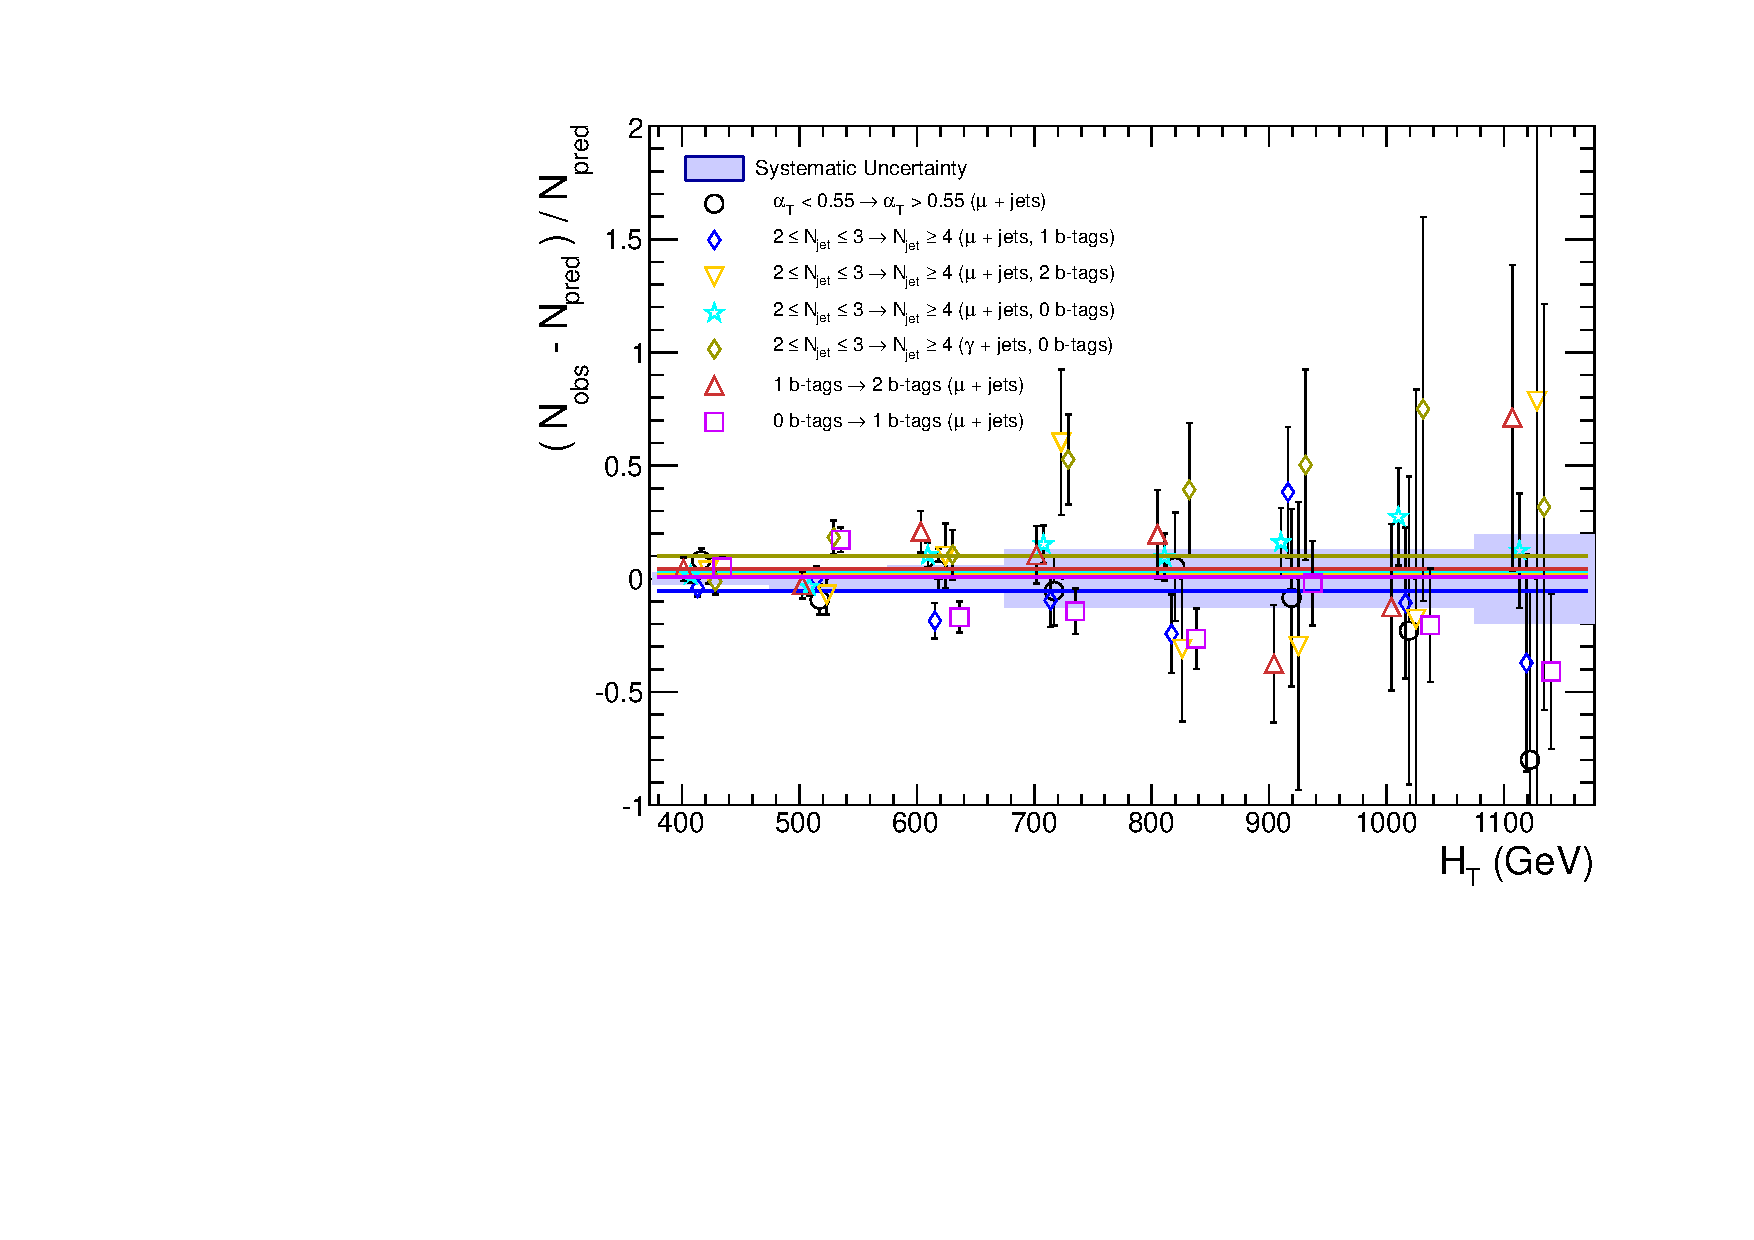
\includegraphics[width=0.7\textwidth]{figures/syst/closureTests_pf_take21_ge4j.pdf}} \\
    \caption{Sets of closure tests (open symbols) overlaid on top of
      the systematic uncertainty used for each of the five \scalht
      regions (shaded bands) and for the two different jet
      multiplicity bins: (a) $2 \leq \njet \leq 3$ and (b) $\njet \geq
      4$.  }
    \label{fig:closure}
  \end{center} 
\end{figure}

%\begin{figure}[h!]
%  \begin{center}
%    \subfigure[$2 \leq \njet \leq 3$ (zeroeth order polynomial fits)]{
%      \includegraphics[width=0.5\textwidth]{figures/syst/v0/le3j/summary_plot_pol0}
%    } 
%    \subfigure[$2 \leq \njet \leq 3$ (first order polynomial fits)]{
%      \includegraphics[width=0.5\textwidth]{figures/syst/v0/le3j/summary_plot_pol1}
%    } \\
%    \subfigure[$\njet \geq 4$ (zeroeth order polynomial fits)]{
%      \includegraphics[width=0.5\textwidth]{figures/syst/v0/ge4j/summary_plot_pol0}
%    } 
%    \subfigure[$\njet \geq 4$ (first order polynomial fits)]{
%      \includegraphics[width=0.5\textwidth]{figures/syst/v0/ge4j/summary_plot_pol1}
%    } \\
%    \caption{Sets of closure tests (open symbols) overlaid on top of
%      the systematic uncertainty used for each of the five \scalht
%      regions (shaded bands), for the two different jet multiplicity
%      bins (top row) $2 \leq \njet \leq 3$ and (bottom row) $\njet
%      \geq 4$, and with zeroeth (left column) and first (right column)
%      order polynomial fits to each set of closure tests. }
%    \label{fig:closure-fits}
%  \end{center} 
%\end{figure}
%
%The first three sets of closure tests are carried out within the $\mu$
%+ jets sample. The first set (indicated by circles) probes the
%modelling of the \alphat distribution in genuine \met events as a
%function of \scalht. This is important to verify the approach of using
%\mj and \mmj samples without an \alphat requirement to make background
%predictions in the signal region, as described in
%Sec.~\ref{sec:larger}. The tests confront data yields in the \mj
%sample with an \alphat requirement against predictions determined in a
%\mj sample with the \alphat requirement inverted. As usual,
%corresponding expectations from simulation are obtained to construct
%the transfer factors required to make the predictions.
%
%The second (times symbols) and third (squares) sets probe the
%sensitivity of the transfer factors to the relative admixture of
%events from the $W$ + jets and \ttbar processes. These tests are
%extremely conservative, as the admixture changes little between the
%\mj sample and the signal region, whereas the closure tests use
%sub-samples with very different admixtures of W + jets and \ttbar
%events. \eg, the former uses a W-enriched sub-sample (selected by
%requiring zero b-jets) to predict yields in a \ttbar-enriched
%sub-sample (selected by requiring one b-jet). These two tests also
%probe the modelling of the reconstruction of b-quark jets, although
%this is also addressed more fully by dedicated studies that determine
%systematic uncertainties via the method described in
%Sec.~\ref{sec:btag-syst}.
%
%The fourth set (triangles), connecting the $\mu$ + jets and $\mu\mu$ +
%jets control samples, again addresses the modelling of the relative
%contributions of $Z$ + jets to $W$ + jets and \ttbar events. This set
%of tests is again a very conservative probe of the sensitivity of the
%transfer factors to the W + jets and \ttbar admixture. At some
%level, the muon trigger and reconstruction efficiencies are probed
%too, given that exactly one and two muons are required in the two
%control samples. However, dedicated data-driven methods are used to
%measure the muon trigger and reconstruction efficiencies, with values
%taken from the muon POG.
%
%The fifth set (crosses) deals with the consistency between the
%Z$\rightarrow\mu\mu$ + jets and $\gamma$ + jets samples, which is an
%important self-consistency cross-check between two independent methods
%used to predict the same irreducible background of \znunu + jets
%events. Hence, this is also an important check on the validity of
%using the \gj process to predict the \znunu\, + jets process.
%%, for which a 20\% theoretical uncertainty on the ratio of
%%cross-sections is assumed~\cite{PAS-SUS-08-002,Bern:2011pa}.
%
%The sixth, seventh and eighth tests probe the simulation modelling of
%the jet multiplicity in the \mj (stars), \mmj (inverted triangles),
%and \gj (diamonds) samples, which is checked due to the exclusive
%binning in jet multiplicity. As in the case of the W + jets / \ttbar
%admixture, this set of tests is a very conservative check, as
%predictions are always made from the same jet multiplicity bin,
%whereas the closure tests translate between the two bins.
%
%In summary, each set of closure tests demonstrate, within the
%statistical precision of each test, that there are no significant
%biases or dependencies on \scalht inherent in the transfer factors
%obtained from simulation. This is demonstrated by
%Tables~\ref{tab:syst-fits-le3j} and \ref{tab:syst-fits-ge4j}, which
%summarise the results obtained from fits of zeroeth order polynomials
%(\ie a constant) to the (five) sets of closure tests performed in both
%the \njetlow and \njethigh bins,
%respectively. Table~\ref{tab:syst-fits-njet} lists the same
%information for the three closure tests performed between the
%different \njet bins. The best fit value and its uncertainty is listed
%for each set of closure tests, along with the $\chi^{2}$, the number
%of degrees of freedom, and the p-value of the fit. The best fit value
%for the constant parameter is indicative of the level of closure, as
%averaged across the full \scalht range considered in the analysis, and
%the p-value is indicative of whether there is any significant
%dependence on \scalht.  
%%The best fit values of all tests are either statistically compatible
%%with zero bias (\ie, less than 2$\sigma$ from zero) or at the level of
%%10\% or less.
%
%Only one set of tests indicates a poor goodness of fit (indicated by a
%low p-value), which is the $\nb = 0 \ra \nb = 1$ test in the \mj
%sample for the \njethigh category, which has been identified as a
%upward (downward) fluctuation of event counts in the \scalht bin
%475--575\gev (575--675\gev) when $\nb = 1$. Combining these two bins
%yields an acceptable fit result, as indicated in
%Table~\ref{tab:syst-fits-ge4j}, which points to a simple fluctuation
%rather than any systematic bias.
%
%In addition to the fits described above, linear fits are also
%performed. The best fit values for the slope terms and the $p$-values
%obtained from each fit are summarised in
%Tables~\ref{tab:syst-fits-le3j}, \ref{tab:syst-fits-ge4j}, and
%\ref{tab:syst-fits-njet}. Typically, the best fit values are of the
%order $10^{-4}$, which corresponds to a percent-level change per
%100\GeV.
%%However, in all cases, the best values values are fully compatible
%%with zero (within 1$\sigma$), indicating that the level of closure is
%%\scalht-independent. 
%Figure~\ref{fig:closure-fits} shows the same information as
%Figure~\ref{fig:closure} but with the zeroeth- and first-order
%polynomial fits superimposed in each figure.
%
%\begin{table}[!h]
%  \caption{A summary of the results obtained from fits of zeroeth
%    order polynomials (\ie a constant) to five sets of closure tests
%    performed in the \njetlow bin. The final two columns show the best
%    fit value for the slope obtained when performing a linear fit and
%    the $p$-value for the linear fit.}
%  \label{tab:syst-fits-le3j}
%  \centering
%  \footnotesize
%  \begin{tabular}{ llrccccrc }
%    \hline
%    \hline
%                                              &          & \multicolumn{4}{c}{Constant fit} &          & \multicolumn{2}{c}{Linear fit}                        \\
%    \cline{3-6}\cline{8-9}                                                                  
%    Closure test                              & Symbol   & Best fit value                   & $\chi^2$ & d.o.f. & $p$-value &  & Slope ($10^{-4}$) & $p$-value \\
%    \hline                                                                                                                                  
%    $\alphat < 0.55 \ra \alphat > 0.55$ (\mj) & Circle   & $-0.02 \pm 0.01$                 & 11.3     & 10     & 0.34      &  & $-2.9 \pm 1.1$    & 0.83      \\ 
%    0 b-jets \ra 1 b-jet (\mj)                & Times    & $ 0.04 \pm 0.01$                 & 5.8      & 10     & 0.83      &  & $-1.5 \pm 0.9$    & 0.97      \\ 
%    1 b-jet \ra 2 b-jets (\mj)                & Square   & $-0.03 \pm 0.02$                 & 5.3      & 10     & 0.87      &  & $-3.0 \pm 1.7$    & 0.99      \\ 
%    \mj \ra \mmj                              & Triangle & $ 0.03 \pm 0.02$                 & 12.3     & 10     & 0.27      &  & $-1.3 \pm 1.1$    & 0.28      \\ 
%    \gj \ra \mmj                              & Cross    & $-0.02 \pm 0.03$                 & 3.0      & 7      & 0.88      &  & $ 0.0 \pm 2.7$    & 0.81      \\ 
%    \hline
%    \hline
%  \end{tabular}
%\end{table}

\begin{table}[!h]
  \caption{\njetlow bin. }
  \label{tab:syst-fits-le3j}
  \centering
  \footnotesize
  \begin{tabular}{ llrccc }
    \hline
    \hline
    &             & \multicolumn{4}{c}{Constant fit} \\
    \cline{3-6}
    Closure test  & Symbol & Best fit value & $\chi^2$ & d.o.f. & $p$-value \\
    \hline
    $\alphat < 0.55 \ra \alphat > 0.55$ (\mj) & Circle & $0.007 \pm 0.02$ & 3.91 & 7 & 0.79 \\ 
    \njetlow \ra \njethigh (\mj, 1 b-tags) & Times & $-0.053 \pm 0.03$ & 8.02 & 7 & 0.33 \\ 
    \njetlow \ra \njethigh (\mj, 1 b-tags) & Invert. Triangle & $0.018 \pm 0.04$ & 6.23 & 7 & 0.51 \\ 
    \njetlow \ra \njethigh (\mj, 0 b-tags) & Star & $0.034 \pm 0.02$ & 9.24 & 7 & 0.24 \\ 
    \njetlow \ra \njethigh (\gj, 0 b-tags) & Diamond & $0.100 \pm 0.04$ & 12.20 & 7 & 0.09 \\ 
    1 b-tags \ra 2 b-tags (\mj, nJet=3) & Triangle & $-0.008 \pm 0.04$ & 3.20 & 7 & 0.87 \\ 
    0 b-tags \ra 1 b-tags (\mj, nJet=2) & Cross & $0.111 \pm 0.03$ & 5.87 & 7 & 0.55 \\ 
    0 b-tags \ra 1 b-tags (\mj, nJet=3) & Square & $0.040 \pm 0.02$ & 1.12 & 7 & 0.99 \\ 
    \hline
    \hline
  \end{tabular}
\end{table}

\begin{table}[!h]
  \caption{\njethigh bin. }
  \label{tab:syst-fits-ge4j}
  \centering
  \footnotesize
  \begin{tabular}{ llrccc }
    \hline
    \hline
    &             & \multicolumn{4}{c}{Constant fit} \\
    \cline{3-6}
    Closure test  & Symbol & Best fit value & $\chi^2$ & d.o.f. & $p$-value \\
    \hline
    $\alphat < 0.55 \ra \alphat > 0.55$ (\mj) & Circle & $0.011 \pm 0.04$ & 5.81 & 7 & 0.56 \\ 
    \njetlow \ra \njethigh (\mj, 1 b-tags) & Times & $-0.053 \pm 0.03$ & 8.02 & 7 & 0.33 \\ 
    \njetlow \ra \njethigh (\mj, 1 b-tags) & Invert. Triangle & $0.018 \pm 0.04$ & 6.23 & 7 & 0.51 \\ 
    \njetlow \ra \njethigh (\mj, 0 b-tags) & Star & $0.034 \pm 0.02$ & 9.24 & 7 & 0.24 \\ 
    \njetlow \ra \njethigh (\gj, 0 b-tags) & Diamond & $0.100 \pm 0.04$ & 12.20 & 7 & 0.09 \\ 
    1 b-tags \ra 2 b-tags (\mj) & Triangle & $0.045 \pm 0.03$ & 9.36 & 7 & 0.23 \\ 
    0 b-tags \ra 1 b-tags (\mj) & Square & $0.007 \pm 0.03$ & 25.30 & 7 & 0.00 \\ 
    \hline
    \hline
  \end{tabular}
\end{table}



%
%\begin{table}[!h]
%  \caption{A summary of the results obtained from fits of zeroeth
%    order polynomials (\ie a constant) to five sets of closure tests
%    performed in the \njethigh bin. The final two columns show the best
%    fit value for the slope obtained when performing a linear fit and
%    the $p$-value for the linear fit. $^{\dag} $See text for details
%    on this particular fit.} 
%  \label{tab:syst-fits-ge4j}
%  \centering
%  \footnotesize
%  \begin{tabular}{ llrccccrc }
%    \hline
%    \hline
%                                              &          & \multicolumn{4}{c}{Constant fit} &          & \multicolumn{2}{c}{Linear fit}                        \\
%    \cline{3-6}\cline{8-9}                                                                  
%    Closure test                              & Symbol   & Best fit value                   & $\chi^2$ & d.o.f. & $p$-value &  & Slope ($10^{-4}$) & $p$-value \\
%    \hline                                                                                                                                 
%    $\alphat < 0.55 \ra \alphat > 0.55$ (\mj) & Circle   & $-0.02 \pm    0.02$              & 17.6     & 10     & 0.06      &  & $-3.1 \pm 1.7$    & 0.11      \\ 
%    0 b-jets \ra 1 b-jet (\mj)                & Times    & $-0.06 \pm 0.02$                 & 31.2     & 10     & 0.00      &  & $-4.1 \pm 1.2$    & 0.02      \\ 
%    0 b-jets \ra 1 b-jet (\mj)$^{ \dag}$      & Times    & $-0.05 \pm 0.02$                 & 13.4     & 9      & 0.15      &  & $-3.9 \pm 1.3$    & 0.78      \\ 
%    1 b-jet \ra 2 b-jets (\mj)                & Square   & $ 0.06 \pm    0.02$              & 13.7     & 10     & 0.19      &  & $ 2.5 \pm 1.6$    & 0.28      \\ 
%    \mj \ra \mmj                              & Triangle & $ 0.11 \pm    0.05$              & 4.8      & 10     & 0.90      &  & $ 0.4 \pm 2.7$    & 0.85      \\ 
%    \gj \ra \mmj                              & Cross    & $-0.00 \pm 0.07$                 & 2.3      & 7      & 0.94      &  & $-5.3 \pm 4.7$    & 0.99      \\ 
%    \hline
%    \hline
%  \end{tabular}
%\end{table}
%
%\begin{table}[!h]
%  \caption{A summary of the results obtained from fits of zeroeth
%    order polynomials (\ie a constant) to three sets of closure tests
%    (\njetlow \ra \njethigh) that probe the accuracy of the MC
%    modelling of the \njet distribution observed in data, using the
%    three data control samples. } 
%  \label{tab:syst-fits-njet}
%  \centering
%  \footnotesize
%  \begin{tabular}{ llrccccrc }
%    \hline
%    \hline
%           &                   & \multicolumn{4}{c}{Constant fit} &          & \multicolumn{2}{c}{Linear fit}                        \\
%    \cline{3-6}\cline{8-9}
%    Sample & Symbol            & Best fit value                   & $\chi^2$ & d.o.f. & $p$-value &  & Slope ($10^{-4}$) & $p$-value \\
%    \hline                                                                                                            
%    \mj    & Star              & $-0.08 \pm 0.01$                 & 9.3      & 10     & 0.50      &  & $0.6 \pm 0.7$     & 0.48      \\ 
%    \gj    & Inverted triangle & $ 0.09 \pm 0.04$                 & 3.7      & 7      & 0.82      &  & $5.1 \pm 3.2$     & 0.98      \\ 
%    \mmj   & Diamond           & $-0.00 \pm 0.05$                 & 4.7      & 10     & 0.91      &  & $2.5 \pm 2.9$     & 0.92      \\ 
%    \hline
%    \hline
%  \end{tabular}
%\end{table}

\subsection{Systematic uncertainties from closure tests\label{sec:syst-from-closure}}

%Once it is established that no significantly large bias or trend is
%observed for any set of closure tests, then systematic uncertainties
%are determined. The statistical precision of the closure tests is
%considered a suitable benchmark for determining the systematic
%uncertainties that are assigned to the transfer factors, as it is only
%the statistical uncertainties associated with the tests that limit our
%knowledge of whether closure is actually achieved or otherwise.
%
%Independent systematics are determined for seven regions in \scalht,
%as indicated in Table~\ref{tab:syst-values}. For each \scalht region,
%the systematic uncertainty is estimated by taking the quadrature sum
%of the weighted mean and sample variance for the closure tests within
%the given \scalht region. This procedure yields the values quoted in
%Table~\ref{tab:syst-values}.
%
%The effect of uncertainties related to the modelling of b-quark jets
%in simulation on the transfer factors is found to be negligible, at
%the percent level as discussed in Section~\ref{sec:btag-syst}, in
%comparison to the aforementioned \njet- and \scalht-dependent
%systematic uncertainties.
%
\begin{table}[!h]
  \caption{A summary of the magnitude of the systematic uncertainties (\%)
    assigned to the transfer factors, according to \njet and \scalht
    region.}
  \label{tab:syst-values}
  \centering
  \footnotesize
  \begin{tabular}{ ccccccccc }
    \hline
    \hline
            & \multicolumn{7}{c}{\scalht region (GeV)}                                \\
    \cline{2-9}
    \njet   & 375--475 & 475--525 & 525--675 & 675--775 & 775--875 & 875-975 & 1075-1075 & $>1175$ \\
    \hline                                                                                                                                  
    2--3    & 3        & 4        & 5        & 11       & 11       & 16      & 16        & 16     \\
    $\geq$4 & 3        & 4        & 6        & 13       & 13       & 13      & 13        & 20     \\
    \hline                                                                                                                                  
    \hline
  \end{tabular}
\end{table}
%
%Figure~\ref{fig:closure} shows the sets of closure tests overlaid on
%top of grey bands that represent the \scalht-dependent systematic
%uncertainties in Table~\ref{tab:syst-values}. These systematic
%uncertainties are assumed to fully uncorrelated between the different
%b jet multiplicity categories and also the seven \scalht regions,
%which is a conservative approach given that one can expect some
%correlation between adjacent \scalht bins (due to comparable
%kinematics).  This approach of decorrelating the \scalht regions
%should be contrasted against the fits shown in
%Figure~\ref{fig:closure-fits} that do assume a correlated behaviour in
%\scalht.
%% while some fits outside bands, could argue to use correlation. plus
%% fit uncertainties not shown. 
%
%%\subsection{Conservative closure tests and systematic uncertainties\label{sec:conservative}} 
%%
%%As mentioned briefly above, several sets of closure tests are
%%considered to be very conservative, due to the significant differences
%%in background composition and event kinematics between the two
%%sub-samples used in the closure test relative to the (much smaller)
%%differences between each control sample and the corresponding
%%background(s) in the signal region. The accurate mirroring of the
%%signal region and control samples is due to kinematically-similar
%%event selections and the fact that the predictions are always made
%%using the same (\njet, \nb, \scalht) bin. Conversely, suitable
%%examples of conservative closure tests are: the two tests that change
%%the \nb requirement (within the \mj sample), the test that uses the
%%\mj and \mmj samples, and the three tests that change the \njet
%%requirement (for each control sample).
%%
%%Consequently, the systematics derived from these conservative closure
%%tests are also considered to be conservative. One important test of
%%this statement is the sensitivity of the transfer factors to the
%%admixture of W + jets and \ttbar in the signal region and \mj control
%%sample. This is demonstrated by Fig.~\ref{fig:vary-xs-le3j} in
%%Appendix~\ref{app:vary-xs}, which shows the effect of varying the
%%cross sections of the W + jets and \ttbar by by $+$20\% and $-$20\%,
%%respectively, on the closure tests performed in the \njet multiplicity
%%bin \njetlow. Similarly, Fig.~\ref{fig:vary-xs-ge4j} shows the effect
%%in the \njet multiplicity bin \njethigh. This variation in cross
%%sections (in opposite directions) is considered to be extreme and is
%%motivated (loosely) by the uncertainty on the experimental
%%measurements of the W + jets and \ttbar inclusive cross sections.
%%
%%Given these variations in cross sections, the level of closure for
%%several tests is subsequently degraded significantly and introduces
%%apparently significant biases. However, the effect on the transfer
%%factors used in the analysis (to ``translate'' an observation in a
%%control sample to a prediction in the signal region) is negligible due
%%to the ``mirroring'' of the signal region and control
%%samples. Table~\ref{tab:vary-xs} demonstrates this by showing the
%%effect on the transfer factors used to predict the W + jets and
%%\ttbar backgrounds when varying the cross sections of W + jets and
%%\ttbar by $+$20\% and $-$20\%, respectively. (In this case, no
%%requirement is made on \njet, but the same behaviour is observed for
%%the exclusive \njet bins.) While the artificial biases introduced to
%%the closure tests are as large as $\sim$30\%, most apparent in the
%%lowest \scalht bins, the effect of the transfer factors used in the
%%analysis is typically at the percent level and only as large as
%%$5\%$. 
%%
%%Hence, given the robust behaviour of the transfer factors with
%%respect to large (and opposite) variations in the W + jets and \ttbar
%%cross sections, one can assume with confidence that any bias in the
%%transfer factors is adequately (and conservatively) covered by the
%%systematic uncertainties -- of at least 10\% -- used in the analysis.

